
\chapter{Limpieza de datos: extracción de usuarios relevantes}
\label{chap:extraccion_de_usuarios}

Como hemos visto en el análisis exploratorio inicial de los datos, la fase 
de limpieza de la información va a ser muy relevante para conseguir
nuestro objetivo final. Se trata de extraer, a partir de los tuits almacenados, 
una lista de usuarios que pudieran constituirse en candidatos adecuados a 
una oferta de trabajo (como, por ejemplo, las de la figura \ref{fig:ofertas_descripcion}). 
Para ello, de todos aquellos usuarios de los que tenemos constancia en 
los tuits recogidos, hemos de seleccionar aquellos que sean personas (eliminando bots, 
empresas, etc.) y que hayan publicado contenido relacionado con la materia de referencia, 
en este caso la ciencia de datos.

Esquemáticamente, el proceso descrito en este capítulo es el siguiente:
\begin{enumerate}
\item Consideramos todos los tuits que hemos descargado, tanto los originales como los datos de los tuits que han sido retuiteados o citados en los originales.
\item Estudiamos los idiomas en que han sido escritos, y seleccionamos aquellos que usaremos en el 
análisis (sección \ref{sect:deteccion_idioma}).
\item Discriminamos los tuits cuyo contenido está relacionado con la ciencia de datos o el Big Data (los \lq\lq relevantes\rq\rq,  sección \ref{sect:tuits_relevantes}).
\item Consideramos los usuarios que han producido esos tuits de contenido relevante, quitando los repetidos
de forma consistente con el resto del proceso (ver detalles en la subsección \ref{subsect:duplicados1}). 
\item De los usuarios relevantes, seleccionamos aquellos que clasificamos como personas (sección 
\ref{sect:tipo_de_usuario}).
\item De aquellos usuarios clasificados como personas, de nuevo eliminamos los duplicados,
según el criterio expuesto en la sección \ref{subsect:duplicados2}.
\end{enumerate}

El resultado de este proceso será entonces una tabla de id de usuarios que procederemos más tarde
a ordenar en función de su relevancia.

Los desarrollos descritos en este capítulo están en el fichero {\bf user\_selection.py}, 
que puede encontrarse en el repositorio de GitHub.


\section{Detección del idioma} 
\label{sect:deteccion_idioma}

El primer paso para poder analizar el contenido de un tuit y determinar si dicho tuit 
(y por tanto el usuario que lo ha publicado) está relacionado con la ciencia de datos o el big data,
es determinar el lenguaje en el que está escrito. Como ya hemos mencionado,
aunque la búsqueda en Twitter se realizó solicitando el campo \lq\lq languages = ["es"]\rq\rq,
obtenemos algunos tuits en otros idiomas, como estos dos 
que mostramos a continuación:

\myfigure{
\begin{tabular}{cc}

\includegraphics[width=0.4\textwidth]{tuit_ingles1}
&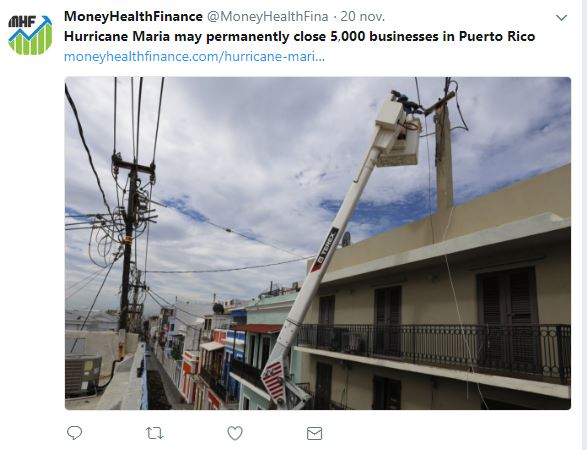
\includegraphics[width=0.4\textwidth]{tuit_ingles2}
\end{tabular}
\figcaption{Tuits no solo en español.}
\label{fig:tuits_ingles} }

Los primeros trabajos sobre el problema de la detección automática del lenguaje de un texto
se remontan a la década de 1970 \cite{zissman-berkling}. En la mayoría de las propuestas, 
existe una fase de entrenamiento, sobre textos previamente clasificados, en la que se produce 
un modelo del lenguaje (tal vez uno por lenguaje), y una fase de reconocimiento, en la que 
el lenguaje de mayor verosimilitud para el texto se extrae a partir de la aplicación de los 
distintos modelos. La clave de todos estos métodos es la modelización del lenguaje, algo que puede 
conseguirse atendiendo a diversas características diferenciadoras: fonemas, morfología, 
sintaxis y/o prosodia. 

La aplicación de dichas técnicas a textos provenientes de entornos web, blogs,  foros, etc. 
no está exenta de problemas, ver por ejemplo \cite{almeida_estevez_piad}.
Los textos procedentes de entornos web en general, y de Twitter en particular, 
presentan elevados niveles de lo que podríamos denominar como \lq\lq ruido\rq\rq,
por ejemplo:
\begin{itemize}
\item suelen ser textos cortos, lo que dificulta la aplicación de técnicas basadas en frecuencia 
de palabras o caracteres,
\item presencia de enlaces web, etiquetas, emoticonos y otros caracteres propios del entorno,
\item uso de jerga, lenguaje informal y palabras en idiomas distintos del principal del texto,
\item modificaciones de la ortografía, que van desde palabras abreviadas (\lq\lq q\rq\rq, 
\lq\lq xa\rq\rq) a expresiones enfáticas (\lq\lq mooooooolaaaaaaaa\rq\rq), por poner dos 
ejemplos.
\end{itemize}


A pesar de que es posible encontrar corpus de textos con estas características 
ya clasificados por 
idioma\footnote{\url{https://blog.twitter.com/engineering/en_us/a/2015/evaluating-language-identification-performance.html }}
que pudieran servir para entrenar un modelo que determinara el lenguaje,
hemos optado por usar un clasificador que no necesite entrenar un modelo, 
ya que esta parte del proyecto no es la principal. Hemos encontrado
referencias, como \cite{almeida_estevez_piad}, que apuntan al buen comportamiento de 
clasificadores que no depende de conjuntos de entrenamiento (basados en \lq\lq small words\rq\rq,
también denominadas \lq\lq stop words\rq\rq, y trigramas). Pero este método requiere de una implementación
{\em ad-hoc}, y las opciones disponibles, listas para usar, nos han parecido lo suficientemente
buenas para el objetivo que perseguimos en este apartado.


En el entorno de Python, hemos encontrado varios paquetes que tratan el 
problema de detectar el idioma de un texto automáticamente. Los más
comentados son los siguientes:
\begin{itemize} 
\item {\tt langid} \cite{langid}: es un paquete que proporciona un 
clasificador Naïve Bayes de textos, que usa $n$-gramas (secuencias de $n$ caracteres en el texto, con $1\leq n\leq 4$). 
El clasificador está pre-entrenado sobre diversos corpus de texto, en un total de 97 idiomas. Según los
resultados explicados en el artículo de presentación del trabajo, es un método con una
exactitud ({\em accuracy}) del 94\%.
\item {\tt langdetect}: de Nakatani Shuyo, también es un clasificador Naïve Bayes basado en $n$-gramas, con
normalizaciones heurísticas, \url{https://github.com/shuyo/language-detection }.
\item {\tt LDIG}: es un clasificador específico para Twitter, creado por el autor
de {\em lagdetect} para solventar las carencias de éste en la clasificación de mensajes
cortos, \url{https://github.com/shuyo/ldig }. Soporta menos idiomas que los anteriores.
\item {\tt equilid}: es el paquete de más reciente creación que hemos encontrado,
que además está especialmente diseñado para tratar el \lq\lq ruido\rq\rq
que comentábamos caracteriza los textos de Twitter. Está concebido para identificar
dialectos urbanos y tratar correctamente expresiones de jerga.
\end{itemize}

Dado el tema que nos ocupa, relacionado con ciencia de datos, la especialización 
de {\tt equilid} y la dificultad de su instalación en el sistema disponible
(usa una versión de TensorFlow que aparentemente no está desarrollada para Windows),
nos hace descartarlo de entrada. 
En \cite{langid2} se muestra que el comportamiento de cualquiera de los clasificadores 
restantes es lo suficientemente bueno por
separado para el objetivo de este proyecto. Sugieren que combinar dos o más clasificadores
puede mejorar la exactitud de la clasificación, y que en general, la limpieza de
los tuits (urls, etiquetas, menciones, etc.), si bien mínimamente en algunos casos,
suele mejorar el comportamiento de los modelos (excepto en el caso de {\tt langid}). 
Finalmente, nos hemos decidido por usar el algoritmo del paquete {\tt langid}, visto
el buen resultado reportado, y la facilidad de uso del mismo. 

En \cite{langid2} se muestra que, en un contexto general de detección del lenguaje, 
el paquete {\tt langid} no parece beneficiarse de una limpieza del tuit
para retirar urls, menciones, etiquetas y emoticonos del cuerpo del mensaje.
Sin embargo, dado que la implementación de esa limpieza no 
es difícil, hemos comparado la clasificación del lenguaje obtenido
con el texto original y con el texto limpio, y hemos observado que en los
textos de los $24,128$ tuits descargados (contando retuiteados y citados también)
hay un $6.37$\% de tuits que no tienen la misma asignación de lenguaje. 
Estos tuits suelen ser tuits con pocas palabras
o con mucha mezcla de idiomas (generalmente español e inglés).

Como método alternativo, se ha implementado un clasificador manual que solo
usa \lq\lq stop words\rq\rq para tratar esos casos en los que {\tt langid}
no da una elección clara del idioma. Si el método de los \lq\lq stop words\rq\rq
da un idioma para el texto que coincide con alguno de los proporcionados por 
{\tt langid} (bien el del texto limpio, bien el del texto original), ese será
el que se asigne al tuit. Y si no, lo dejaremos clasificado con un idioma desconocido.

Hemos aplicado este método de clasificación del lenguaje a los $24,128$ textos
de los tuits originales, retuiteados o citados, y resulta una clasificación en $25$
idiomas diferentes. Mostramos a continuación un resumen de los resultados del clasificador:


\myfigure{
\begin{tabular}{cc}
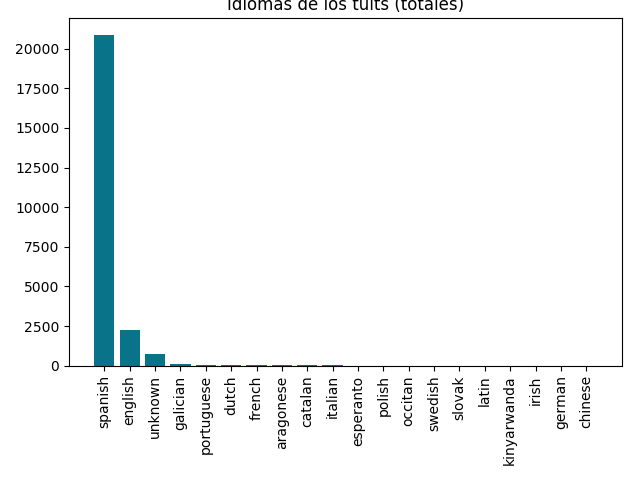
\includegraphics[width=0.4\textwidth]{C:/DATOS/MBIT/Proyecto/MBITProject_Data4all/Python/images/assigned_languages.png}
&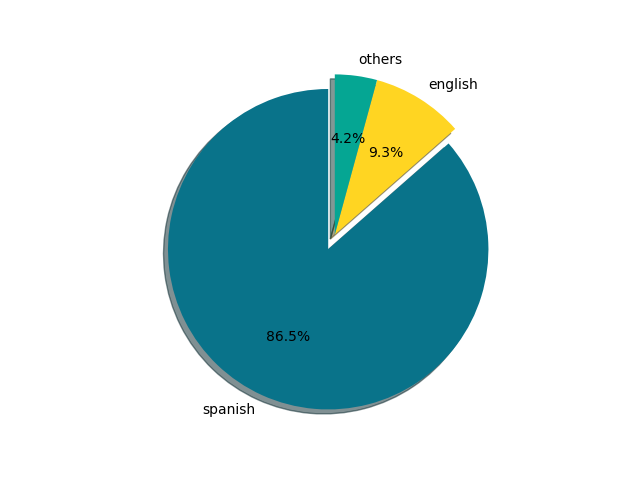
\includegraphics[width=0.4\textwidth]{C:/DATOS/MBIT/Proyecto/MBITProject_Data4all/Python/images/assigned_languages_proportions.png}
\end{tabular}
\figcaption{Clasificación por lenguaje del texto del tuit. Del $4.2$\% de \lq\lq others\rq\rq
hay un $2.9$\% de \lq\lq unknown\rq\rq. ¿Errores de clasificación?}
\label{fig:assigned_languages} }

Echando un vistazo a los resultados, aquellos que no están clasificados o que están
clasificados en idiomas poco probables, digamos, como el esperanto, son aquellos en los
que el clasificador seguramente ha fallado. Algunas veces parece ser porque casi no 
tuvieran texto o porque el texto contenga mucha mezcla de idiomas. Pero otras veces, 
como en el siguiente caso clasificado en esperanto, no está muy claro por qué:

\myfigure{
\begin{tabular}{cc}

\includegraphics[width=0.8\textwidth]{tuit_esperanto1}
\end{tabular}
\figcaption{Tuit clasificado como esperanto.}
\label{fig:tuit_esperanto1} }


{\bf Vistos los resultados del clasificador de lenguaje, usaremos para el análisis del contenido de los tuits
los idiomas inglés y español.}

\section{Naturaleza del tuit}
\label{sect:tuits_relevantes}
texto del tuit:  IT, cientifico, analista o nodatascience (diccionarios de palabras)
					/Binario, data science o no data science


\subsection{Listado de usuarios únicos}
\label{subsect:duplicados1}

El resultado del proceso que acabamos de describir
es una lista de tuits clasificados como relevantes o no relevantes
para nuestro propósito (encontrar candidatos para un puesto de científico de datos).
Nos quedaremos naturalmente solo con aquellos que hayamos clasificado como relevantes.

En esta lista de tuits relevantes, es razonable esperar que haya algunos 
publicados por el mismo usuario. Para optimizar la ejecución
del siguiente tramo del proceso, la selección de aquellos usuarios que son personas, 
de la lista de usuarios que podemos extraer de aquellos tuits que hemos clasificado como
relevantes, nos vamos a quedar solo con instancias únicas de los usuarios.

A lo largo de los procesos descritos en este capítulo y en el capítulo \ref{chap:ordenacion_de_usuarios},
la referencia que vamos a usar para seguir a los usuarios es el número de identificación 
de usuario de Twitter, al que nos referiremos habitualmente como id.
Sin embargo, no es conveniente en esta etapa del proceso, quitar simplemente los id 
repetidos. Como veremos en la sección \ref{sect:tipo_de_usuario}, los campos relevantes
para la clasificación de un usuario en persona o no persona, son 
la url, el nombre de usuario y la descripción del usuario. Todos estos campos
pueden ser modificados por el usuario, y podría darse el caso de haber descargado
tuits de un mismo usuario, en el que aparecieran diferentes url, nombre de usuario o
descripción.

Dado que un usuario podría clasificarse de forma distinta con diferentes url, nombre de usuario y 
descripción, en esta etapa vamos a considerar que un usuario es un usuario repetido si para dos 
usuarios sus url, nombres de usuario, descripciones y por supuesto sus id, son iguales.

\section{Tipo de usuario}
\label{sect:tipo_de_usuario}
Para clasificar al usuario respecto a su entidad, y por ejemplo distinguir entre personas, bots y empresas, 
una de las partes del tuit que más información contiene, a partir de los datos conseguidos, es
la descripción que los propios usuarios aportan. Antes de cualquier labor de análisis de esos textos,
es necesario saber el idioma en el que están, y por ello de nuevo aplicamos a nuestros datos 
el identificador de lenguaje que usamos en el apartado anterior. 

Primero seleccionamos los datos correspondientes a los usuarios distintos, obteniendo
$7,210$ usuarios con distinto \lq\lq{\em id\_str}\rq\rq. {\tt langid} clasifica de 
forma diferente el idioma de los datos de perfil antes y después de 
limpiarlos (quitar urls, emojis, hashtags, etc.) en un $5.99$\%
de los casos. Después de aplicar en éstos últimos el método de las \lq\lq stop words\rq\rq, 
los perfiles de los usuarios han quedado clasificados en $44$ idiomas diferentes.

\myfigure{
\begin{tabular}{cc}
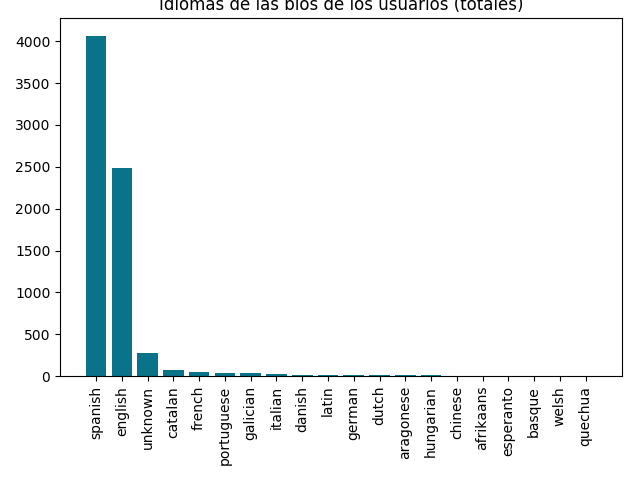
\includegraphics[width=0.4\textwidth]{C:/DATOS/MBIT/Proyecto/MBITProject_Data4all/Python/images/user_bios_assigned_languages.png}
&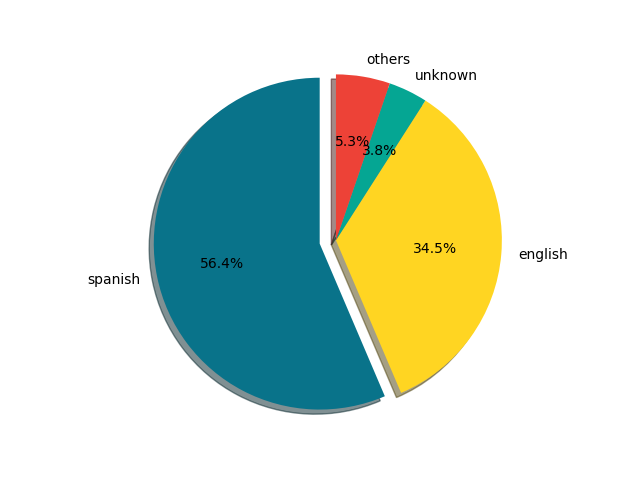
\includegraphics[width=0.4\textwidth]{C:/DATOS/MBIT/Proyecto/MBITProject_Data4all/Python/images/user_bios_assigned_languages_proportions.png}
\end{tabular}
\figcaption{Clasificación por lenguaje del texto de las bios.}
\label{fig:user_bios_assigned_languages} }

{\bf De nuevo, vistos los resultados del clasificador de lenguaje, usaremos para el análisis del tipo 
de usuario los idiomas inglés y español.}

Para poder hacer una ordenación de los candidatos necesitamos detectar a usuarios o personas reales 
y descartar a empresas o tuits automatizados. Hemos investigado en la red algunas técnicas 
para llevar a cabo esta distinción, y hemos decidido seguir la mostrada en \cite{user_class}.
En este trabajo de la Universidad de Utah de 2014, proponen basarse en campos como el nombre de usuario, 
la descripción, la url y el origen de los tweets para clasificar los tuits como publicados por personas 
y resto. Para ello la idea es la siguiente: se considera que un tuit pertenece a una persona si 
cumple las siguientes cuatro especificaciones:
\begin{itemize}
\item[{\bf E1}] En el campo nombre de usuario aparece un nombre que coincida totalmente con un nombre real 
de persona. Para ello hemos manejado un archivo con nombres y apellidos de personas en español e inglés, 
obtenido de estas fuentes:
\begin{itemize}
\item\url{ https://www.census.gov/genealogy/www/%20data/1990surnames/names_files.html }
\item\url{
http://www.ine.es/dyngs/INEbase/es/operacion.htm?c=Estadistica_C&cid=1254736177009&menu=resultados&idp=1254734710990 }
\item\url{http://www.buscanombres.com/nombres-gallegos.htm }
\item\url{https://script.byu.edu/Pages/Spanish/es/surnames.aspx }
\end{itemize}
Para el caso de los nombres españoles se han incluido también los específicos para regiones como Cataluña, Comunidad Valenciana y Galicia.
\item[{\bf E2}]El texto en el campo descripción cumple las siguientes dos condiciones:
\begin{itemize}
\item aparecen palabras como \lq\lq emprendedor\rq\rq, \lq\lq persona\rq\rq, 
\lq\lq profesional\rq\rq o \lq\lq consultor\rq\rq. Se evitó poner las palabras \lq\lq I am\rq\rq o 
\lq\lq soy\rq\rq porque en el caso de algunos bots, en este campo aparecen textos
similares a \lq\lq I am a bot\rq\rq. 
\item En el campo descripción y el el campo nombre, no aparecen palabras relativas a empresas como 
\lq\lq negocio\rq\rq, \lq\lq empresa\rq\rq, \lq\lq compañía\rq\rq,\lq\lq somos\rq\rq, \lq\lq we\rq\rq\dots.
En este último caso también se creo un fichero con todas estas palabras relacionadas con empresas, 
en inglés y en español. Se evitaron palabras como \lq\lq business\rq\rq por riesgo a que algunos pudieran 
publicar comentarios del área de {\em business intelligence}.
\end{itemize}
\item[{\bf E3}] Si el campo de url estaba vacío, asignar la categoría de persona y no de empresa (o bot).
\item[{\bf E4}] Considerar el origen del tweet: las empresas no suelen publicar tweets desde dispositivos de mano. 
\end{itemize}

Al intentar aplicar esta metodología, observamos lo siguiente:
\begin{itemize}
\item Hay más empresas de las que cabría esperar, y fundamentalmente bots, cuyo campo url estaba vacío. No
nos parece entonces una buena característica para la clasificación. Sin embargo, sí que se atendió al hecho 
de que a veces en el campo url el usuario incluye en este campo su perfil de LinkedIn (con lo que el
texto \lq\lq linked\rq\rq aparece) o su blog personal (en cuyo caso podemos identificar el texto 
\lq\lq blog\rq\rq). Es cierto que en el caso de \lq\lq blog\rq\rq se puede incurrir en ciertos errores,
dado que también hay bots en cuyo campo url se incluye un blog y es uno de los puntos a mejorar. 
\item La idea apuntada en la subsección sobre el origen de los tuits en la
página \pageref{subsubsect:origen_tuits}, que si el tuit era publicado desde un dispositivo de mano 
probablemente se trataría de una persona,  finalmente resultó que, de nuevo, no era la realidad y esa
diferenciación no era tan clara. 
\item En cuanto al campo nombre de usuario, a pesar de la amplia lista de nombres y apellidos,
en muchos casos solo se identificaba el nombre, en otros solo los apellidos... Con lo que en lugar de validar a las personas con la coincidencia completa de su nombre de usuario, se determinó 
aceptar que es un nombre válido si se da una coincidencia del $33$\%. En aquellos casos en los que una 
persona incluye solo nombre y apellidos, sería suficiente con dejar el corte en el $50$\%,
pero cuando se publican nombre y dos apellidos,  es frecuente que solo detectemos el nombre y no los apellidos. De ahí que se tomara la decisión de fijar el umbral en el $33$\%.
\item Con los criterios {\bf E1} y {\bf E2} se conseguía una buena clasificación de empresas y de personas. 
Los fallos fundamentales de usuarios reales provenían de tuits con nombres de usuario extraños y descripciones
ambigüas, y fundamentalmente bots de diferentes tipos.
\end{itemize}

En vista de todas estas observaciones, el algoritmo que hemos usado toma la siguiente forma:
un tuit se considera de una persona cuando en su campo nombre de usuario existe un $33$\% o más 
de coincidencia con la lista de nombres y apellidos, y además tanto en su campo nombre de usuario 
o descripción no aparecen términos relacionados con empresa, o bien cuando su url es una 
url de LinkedIn o de un blog.

Aplicando esta metodología a la lista de usuarios únicos obtenidos tras la aplicación
de los algoritmos descritos en la sección \ref{sect:tuits_relevantes}, 
hemos obtenido los siguientes datos: de los tantos:cambiar usuarios únicos, 
hay tantos:cambiar que han sido clasificados como persona. De éstos, había tantos:cambiar
cuya id es única (es decir, había tantos:cambiar cuyo nombre de usuario, url o descripción ha cambiado
en los tuits descargados). Los resultados relativos están consignados en la siguiente gráfica:

\myfigure{
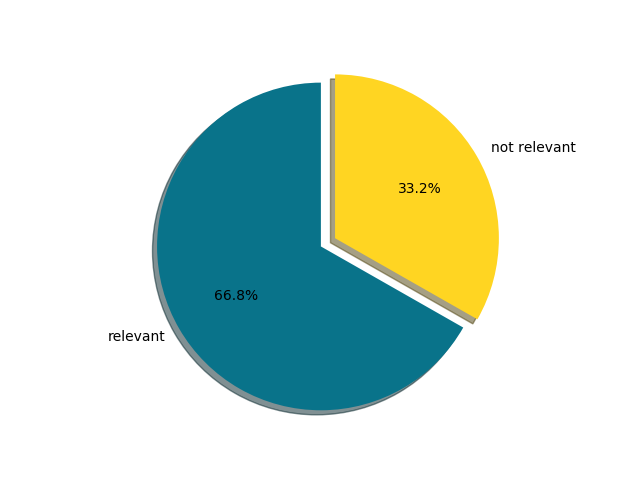
\includegraphics[width=0.6\textwidth]{C:/DATOS/MBIT/Proyecto/MBITProject_Data4all/Python/images/relevant_users_proportion.png}
\figcaption{Porcentaje de usuarios clasificados como personas.}
\label{fig:} }

El código para llevar a cabo esta limpieza estaría preparado para escalar
el modelo a otros casos de uso. Por ejemplo:
\begin{itemize}
\item la lista de nombres y apellidos puede extenderse fácilmente para incluir nombres
en otros idiomas, si resulta que el texto de las descripciones o de los tuits recolectados
se clasifica en otros lenguajes además del inglés y el español, o para extender el alcance de
detección del modelo.
\item De igual forma, en la lista de términos que sí pueden aparecer en descripción, donde ahora
incluimos fundamentalmente vocablos relacionados con perfiles técnicos (consultor, matemático, ingeniero, etc.)
para clasificar los usuarios como personas, se puede modificar fácilmente para incluir aquellos que estén 
relacionados con el perfil requerido en la oferta laboral y mejorar la clasificación.
\item Respecto a la lista de términos que no deben aparecer en el campo descripción (porque identifican empresas 
o bots) se podría utilizar sin ningún cambio. En el caso en el que los tuits sean en otros idiomas diferentes 
al inglés o al español se podría incluir fácilmente la versión en los idiomas necesarios de las palabras 
consideradas.
\end{itemize}

\subsection{Eliminación de duplicados}
\label{subsect:duplicados2}
Una vez obtenida la clasificación en persona o no persona de los usuarios llevada a cabo como
hemos descrito, solamente nos queda producir el listado definitivo de candidatos seleccionados 
(ya no va a haber ninguna clasificación posterior). Esto implica, en primer lugar, que eliminaremos
de la lista aquellos usuarios que no han sido clasificados como persona. A continuación, nos interesa
extraer las personas únicas que hemos detectado: del listado extraído del paso anterior, 
sección \ref{subsect:duplicados1}, podría ocurrir que un usuario  fuera clasificado como persona con un
conjunto de url, nombre de usuario y descripción, pero no lo fuera con otro. En esta fase, por tanto, nos limitaremos a eliminar del listado de los clasificados como personas aquellos usuarios con un id repetido.